\chapter{ARTDroid: Hooking on Android ART Runtime}

To build a better hooking framework for dynamic analysis, we design \textbf{ARTDroid}, an framework for hooking virtual-method calls under the latest Android runtime (ART). The idea of hooking on ART is tampering the virtual method table (vtable) for detouring virtual-methods calls. The vtable is to support the dynamic-dispatch mechanism. And, dynamic dispatch, i.e., the runtime selection of a target procedure given a method reference and the receiver type, is a central feature of object-oriented languages to provide polymorphism. Since almost all Android sensitive APIs are virtual methods, we can collect the apps behavior by using ARTDroid to hook Android APIs methods.

To summarize, this work makes the following contributions.

\begin{itemize}
\item We propose ARTDroid, a framework for hooking virtual-method calls without any modifications to both the Android system and the app's code.
\item We discuss how ARTDroid is made fully compatible with any real devices running the ART runtime with root privilege.
\item We demonstrate that the hooking technique used by ARTDroid allows to intercept virtual-methods called in both Java reflection and JNI ways.
\item We discuss applications of ARTDroid on malware analysis and policy enforcement in Android apps.
\item We released ARTDroid as an open-source project \footnote{\url{https://vaioco.github.io}}. 
\end{itemize}

The rest of this paper is organized as follows. Section \ref{sec:backg} introduces the background about Android and the new Android runtime ART. The ARTDrod framework is introduced in Sec. \ref{sec:artdroid} and its implementation is discussed in Sec. \ref{sec:impl}. Performance evaluation is presented in Sec. \ref{sec:eva}, and discussion and applications are in Sec. \ref{sec:discuss}. Section \ref{sec:related} discuss some related works, and we conclude this paper in Sec. \ref{sec:conclusion}.

\section{Background}
\label{sec:backg}

Android apps are usually written in Java and compiled to Dalvik bytecode (DEX). To develop an Android app, developers typically use a set of tools via Android Software Development Kit (SDK). 

With Android's Native Development Kit (NDK), developers can write native code and embed them into apps. The common way of invoking native code on Android is through Java Native Interface (JNI).


\subsection{ART Runtime}
\label{subsec:art}

ART, silently introduced in October 2013 at the Android KitKat release, applies Ahead-of-Time (AoT) compilation to convert Dalvik bytecode to native code. 

At the installation time, ART compiles apps using the on-device \textbf{dex2oat} tool to keep the compatibility. The {\tt dex2oat} is used to compile Dalvik bytecode and produce an \textit{OAT} file, which replaces Dalvik's \textit{odex} file. 

Even Android framework JARs are compiled by the {\tt dex2oat} tool to the {\tt boot.oat} file. To allow pre-loading of Java classes used in runtime, an image file called {\tt boot.art} is created by dex2oat. The image file contains pre-initialized classes and objects from the Android framework JARs. Through linking to this image, OAT files can call methods in Android framework or access pre-initialized objects. We are going to briefly analyze the ART internals, using as codebase the Android version 6.0.1\_r10.



\begin{figure}[h!]
\lstinputlisting[language=C++]{mysnippets/class.h}
\caption{ART Class type}
\label{lst:artclass}
\end{figure}

The ART runtime uses specific C++ classes to mirror Java classes and methods. Java classes are internally mirrored by using \textbf{Class}\footnote{art/runtime/mirror/class.h}. In Figure \ref{lst:artclass}, virtual-methods defined in \textit{Class} are stored in an array of {\tt ArtMethod*} elements, called {\tt virtual\_methods\_} (line 11). The {\tt vtable\_} field (line 8) is the \textbf{virtual method table}. During the linking, the vtable from the superclass is copied, and the virtual methods from that class either override or are appended inside it. Basically, the vtable is an array of {\tt ArtMethod*} type. Direct methods are stored in the {\tt direct\_methods\_ } array (line 10) and the  {\tt iftable\_} array (line 5) contains pointers to the interface methods. We leave interface-methods hooking for future work. The Figure \ref{art:artmethod} shows the definition of \textbf{ArtMethod} class\footnote{art/runtime/art\_method.h}. The main functionality of {\tt ArtMethod} class is to represent a Java method.


\begin{figure}[h!]
\lstinputlisting[language=C++]{mysnippets/art-method.h}
\caption{ART ArtMethod type}
\label{art:artmethod}
\end{figure}

By definition, a method is declared within a class, pointed by the {\tt declaring\_class\_ } field (line 3). The method's index value is stored in the {\tt method\_index\_ } field (line 5). This value is the method's index in the concrete method dispatch table stored within method's class. The {\tt access\_flags\_ } field (line 4) stores the method's modifiers (i.e., public, private, static, protected, etc\ldots) and the {\tt PtrSizedFields} struct, (line 7), contains pointers to the ArtMethod's entry points. Pointers stored within this struct are assigned by the ART compiler driver at the compilation time. 


\subsection{Virtual-methods Invocation in ART}
\label{subsub:artinvoke}
In this paragraph we describe how ART runtime invokes virtual-methods by choosing the virtual-method {\tt android.telephony.TelephonyManager}'s {\tt getDeviceId} as an example. Figure \ref{fig:es1} shows that the getDeviceId method is invoked on TelephonyManager object's class (line 4). Figure \ref{fig:oatdump} shows dumped compiled codes for arm architecture by \textit{oatdump} tool. 


\begin{figure}[H]
\lstinputlisting[language=Java]{mysnippets/testcode.java}
\caption{Call to method getDeviceId} 
\label{fig:es1}
\end{figure}

\begin{figure}[h!]
\lstinputlisting{mysnippets/compiledcode.txt}
\caption{Compiled native code of callGetDeviceId}
\label{fig:oatdump}
\end{figure}


Before discussions on native code, in Fig. \ref{fig:oatdump}, we briefly introduce the devirtualization. To speedup runtime execution, during the on-device compilation time, virtual-methods calls are devirtualized. Devirtualization process uses method's index to point to the relative element inside the vtable within {\tt receiver} instance's class.  As result, compiled code contains static memory offset used to get the called ArtMethod's memory reference. 
 

Now, we discuss the native code generated for the method \textit{callGetDeviceId}. The line 4 in Figure \ref{fig:es1} is compiled in lines 11-18 in Figure \ref{fig:oatdump}. The TelephonyManager instance (an Object\footnote{art/runtime/mirror/object.h} type) is stored in the register \textit{r2}. Then, the instance's class is retrived from address in \textit{r2} and stored in the register \textit{r0} (line 13). The method getDeviceId (an ArtMethod type) is directly retrived (line 16) from memory using a static offset from address stored in \textit{r0}. Finally, the getMethodId's entrypoint is called using the ARM branch instruction \textit{blx} (line 18). The entrypoint's address is also retrived by using a static memory offset from the ArtMethod reference (line 17). 


In Java, it is allowed to invoke a method dynamically specified using {\tt Java Reflection}. 

Reflection calls managed by ART runtime use the function {\tt InvokeMethod}\footnote{art/runtime/reflection.cc}. This function calls {\tt FindVirtualMethodForVirtualOrInterface} which returns a pointer to the searched method by looking in the {\tt vtable\_} array of receiver's class.


A Java method can also be invoked by native code using the {\tt Call<type>Method } family functions, exposed by JNI. 
For instance, function {\tt CallObjectMethod(JNIEnv* env, jobject obj, jmethodID mid, ...) }\footnote{art/runtime/jni\_internal.cc} is used to call a virtual-method which returns an Object type. When a Java method is invoked from native code using a function from {\tt Call<type>Method } family, the ART runtime will go through the {\tt vtable\_} array to find a matched method matching.


There are two different ways to get a Java virtual-method's reference. One is through the reflection APIs exposed by {\tt java.lang.Class}. For instance, the method {\tt getMethod} returns a reference which represents the public method with a matched method signature. All java.lang.Class' methods, which permits to get a virtual-method reference, can use the {\tt virtual\_methods\_ } array to lookup the requested method. The other way is offered by the JNI function {\tt FindMethodID}. It searches for a method matching both the requested name and signature by looking in the {\tt virtual\_methods\_ } array within the class reference passed as argument.


\section{Framework Design}
\label{sec:artdroid}

The goal of ARTDroid is to avoid both app's and Android system code modifications. So, the design of ARTDroid is oriented towards directly modify the app's virtual-memory tampering with ART internals representation of Java classes and methods.
ARTDroid consists of two components. The first component is the core engine written in C and the other one is the Java side that is a bridge for calling from user-defined Java code to ARTDroid's core. The core engine aims to: find target methods' reference in virtual memory, load user-supplied DEX files, hijack the vtable and set native hooks. Moreover, it registers the native methods callable from the Java side. ARTDroid is configured by reading a user-supplied JSON formatted configuration file containing the target methods list.


Suppose that you want to intercept calls to a virtual-method. You have to define your own Java method and override the target method by using ARTDroid API. All calls to the target method will be intercepted and then go to your Java method (we call it {\tt patch code}). ARTDroid further supports loading \textit{patch code} from DEX file. This allows the “patch” code to be written in Java and thus simplifies interacting with the target app and the Android framework (Context, etc…). 

ARTDroid is based on library injection and uses Android Dynamic Binary Instrumentation toolkit\cite{ADBI} released by Samsung. The ABDI tool is used by ARTDroid to insert trace points dynamically into the process address space. 


ARTDroid requires the root privilege in order to inject the hooking library in the app's virtual memory, and the hooking library can be injected either in a running app or in the Zygote\cite{lee2014zygote} master process.

Now, we explain the framework design in figures. Figure \ref{fig:design1} shows the app's memory layout without ARTDroid. The class \textit{TelephonyManager} is loaded within the boot image (boot.art). This Class contains both the \textit{vtable\_} and \textit{virtual\_methods\_} arrays where the pointer to method getDeviceId is stored. Instead, Figure \ref{fig:design2} represent the app's memory layout while ARTDroid hooking library is enabled. First, the hooking library is loaded inside the app's virtual memory (step 1), and then ARTDroid loads the user-defined patch code by DexClassLoader's methods (step 2). After this, ARTDroid uses its internal functions to retrive target methods reference. So, it can hook these methods by both {\tt vtable\_} and {\tt virtual\_methods\_} hijacking (step 3). \\

\begin{figure}[H]
\centering
   \subfigure[ARTDroid not enabled]{\label{fig:design1}  
   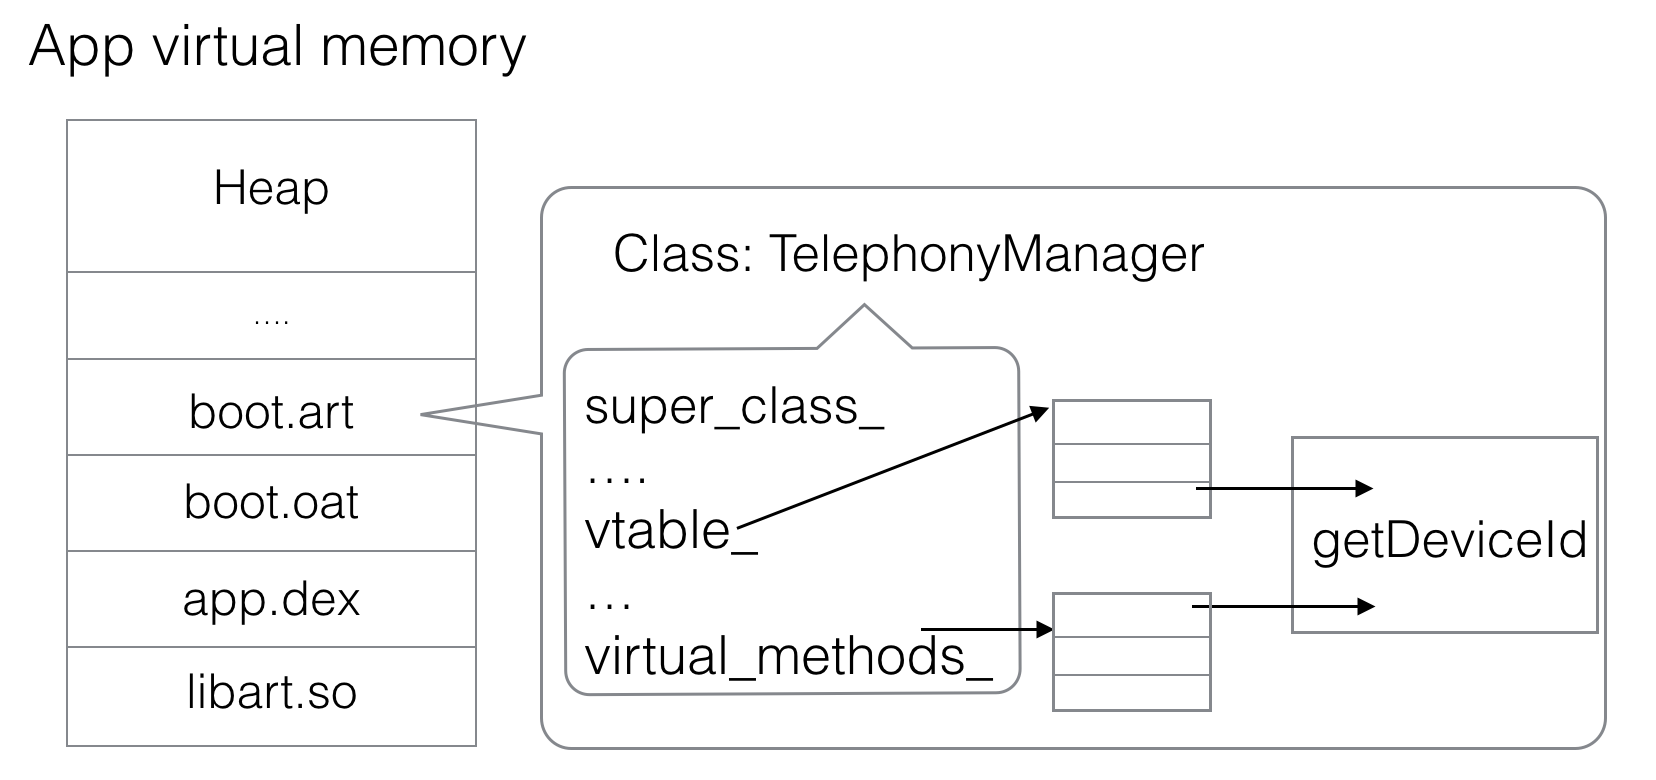
\includegraphics[width=\textwidth]{design1}}
   \subfigure[ARTDroid enabled]{\label{fig:design2}
   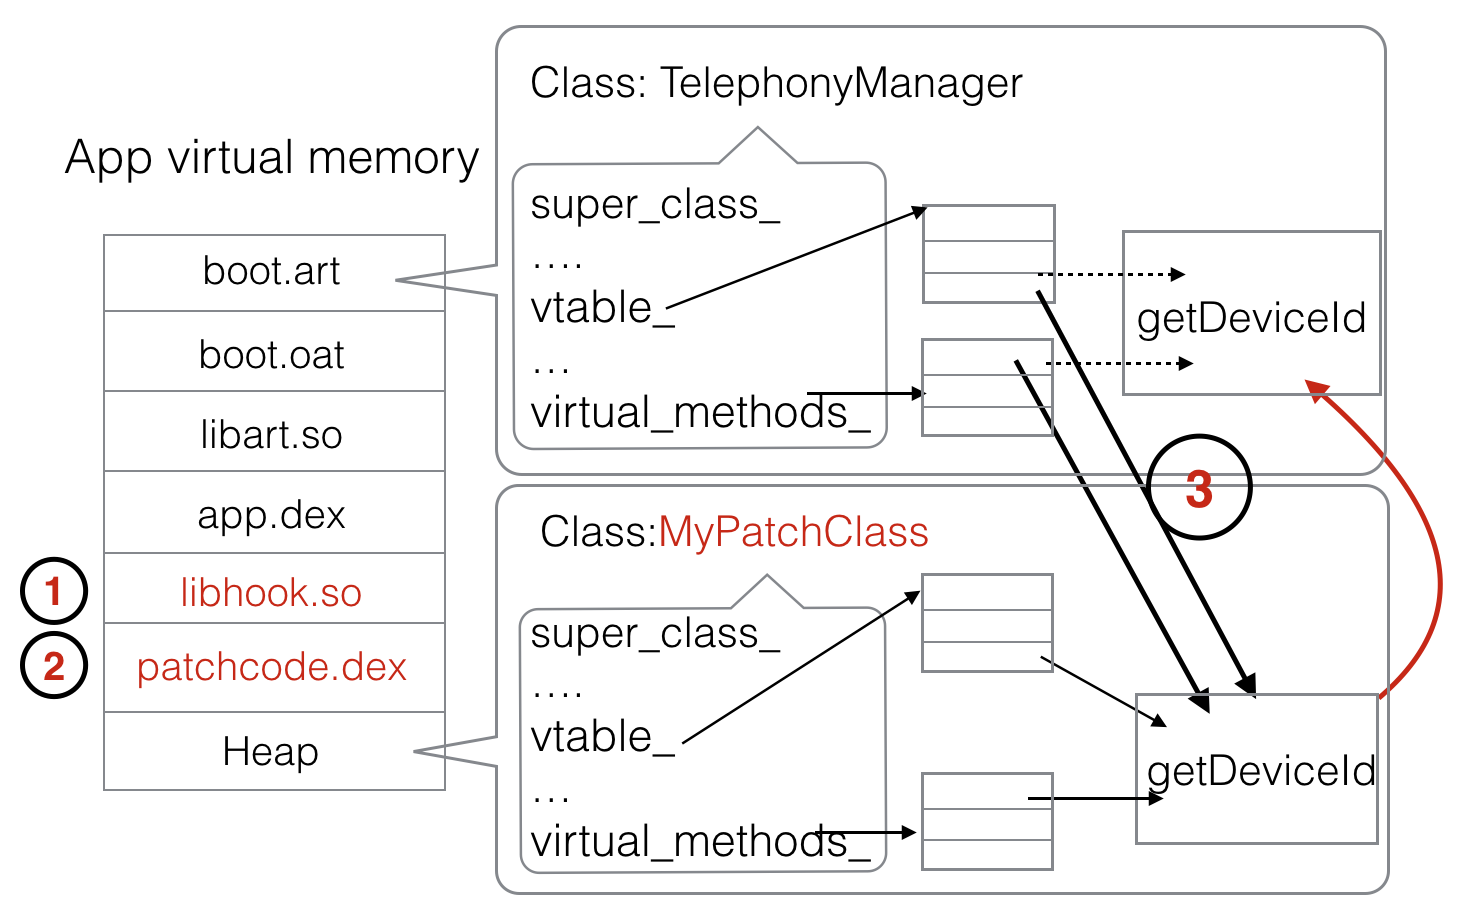
\includegraphics[width=\textwidth]{design2}}
\caption{App virtual memory layout}
\end{figure}



As discussed in \ref{subsub:artinvoke}, the {\tt vtable\_} array is used by the ART runtime to invoke a virtual-method. Instead, the {\tt virtual\_methods\_} array is accessed to return a virtual-method’s reference from memory. ARTDroid exploits these mechanisms to hooking virtual-methods by both {\tt vtable\_ } and {\tt virtual\_methods\_ } hijacking means.



\section{Implementation}
\label{sec:impl}
To get the target method's reference, ARTDroid uses the JNI  function {\tt FindMethodID}. 


ARTDroid overwrites the target method's entry within both the {\tt vtable\_} and {\tt virtual\_methods\_ } array by writing the address of the method's patch code. The original method's reference is not modified by ARTDroid and its address is stored inside the ARTDroid's internal data structures. This address will be used to call the original method implementation. 


When ARTDroid hooks a target method, all calls to that method will be intercepted and they will go to the patch code. Then, the patch code receives the \textit{this} object and the target method's arguments as its parameters. To call the original implementation of target method, ARTDroid exports the function {\tt callOriginalMethod} to the Java patch code. Internally, ARTDroid's core engine calls the original method implementation using the JNI {\tt CallNonVirtual<type>Method} family of routines. These functions can invoke a Java instance method (non-static) on a Java object, according to specified class and methodID.

The original method implementation is invoked by ARTDroid using its address internally stored  before the hooking phase. To guarantee a reliable hooking, ARTDroid uses ADBI features to hook the functions of {\tt CallNonVirtual<type>Method} family. By doing this, all calls to these functions are checked by ARTDroid to block calls to an hooked virtual-method only if these calls do not come from ARTDroid's core engine.


\section{Evaluation}
\label{sec:eva}

\subsection{Performance Test}

To measure the effectiveness of virtual-methods hooking, we firstly need a test set of sensitive methods. SuSi\cite{rasthofer2014machine} provides sensitive methods in Android 4.2. To verify how many of these methods are declared as virtual,  we firstly test them in Android emulator in version 4.2. We use Java reflection to call these methods at runtime. The result of our experiment shows that a remarkable number of virtual-methods could be used to threaten user privacy. The following list describes our experiment results: 

\begin{itemize}
\item 65.1\% of these methods are declared as virtual
\item 6.6\% are non-virtual
\item 28.3\% methods not found
\end{itemize}


Unfortunately, the only methods list available from SuSi is from Android version 4.2. To overcome this limitation, we analyze the sensitive methods list offered by PScout\cite{au2012pscout}. The methods of PScout are available from version 2.2 to version 5.1.1. Our another test is on Android 5.1.1 codebase and it is carried on a Nexus 6 running Android 5.1.1. After analyzing them, we know that only 1.0\% of methods are non-virtual. 

\begin{itemize}
\item 59.2\% of these methods are declared as virtual
\item 1.0\% are non-virtual
\item 39.8\% methods not found
\end{itemize}

However, some methods cannot be found via Java reflection because corresponding classes or methods are not visible to normal apps. They belong to the Android system apps.

So, we can conclude that most of sensitive methods are virtual from our test results. ARTDroid can cover all sensitive methods except 1.0\% methods on Android 5.1.1.



The overhead introduced by ARTDroid depends much on the behavior of the patch code. 

To measure the overhead, we developed a test app, which repeatedly calls sensitive methods or APIs. In particular, this applciation attempts to perform the following operations by calling Android APIs (both via Java reflection and JNI) : initiate several network connections, access sensitive files on the SD card (such as the user's photos), send text message to premium numbers, access the user's contact list and retrive the device's IMEI. 

We used the profiling facilities offered by Android calling the \textit{android.os.Debug}'s \textit{startMethodTracing}/\textit{stopMethodTracing}. Then, the produced traces can be analyzed using either \textit{traceview} or \textit{dmtracedump}. To measure the effective overhead due to ARTDroid, we call the methods using both Java reflection and JNI in addition to the normal invocation. We ran the test 10,000 times for each method, once with ARTdroid disabled and then with ARTDroid enabled mode. The average running time for each call to an hooked method is showed in the following Table \ref{t:perf}.

The most of overhead in ARTDroid is caused by the JNI call, which is internally used to invoke the original method implementation. We registered a worst case overhead of 25\% for each hooked method. Therefore, the total overhead of a call to an hooked method is around 0.25 seconds. This overhead could be decreased by adding an internal cache to store methods' reference called by ARTDroid, instead of using JNI function \textit{FindMethodID}  at each call. We leave these improvements as future work. \\

\begin{table}[ht]
\centering
\caption{Performances}

\bigskip

\begin{tabular}{c  c c c }
\toprule
\multicolumn{1}{c}{ARTDroid} & & Invoke type \\
\cmidrule(r){2-4}
enabled? &  Normal & Reflection & JNI \\ 
\midrule
Yes & 1.12 s   &   1.39 s  &   1.19 s  \\ 
No & 0.88 s& 1.14  s & 0.94 s \\ 
\toprule
overhead & 0.24 s    &   0.25 s  &   0.25 s \\
\toprule
\end{tabular}
\label{t:perf}
\end{table}


\subsection{Case Study}
\label{sec:usage}

Now, we show a case study by hooking \textit{TelephonyManager}'s \textit{getDeviceId} in ARTDroid.

\begin{figure}[ht]
\begin{center}
\lstinputlisting[language=xml]{mysnippets/config.json}
\caption{ARTDroid configuration file}
\label{artconf}
\end{center}
\end{figure}

Figure \ref{artconf} shows the configuration file which contains the definition of methods to hook. 
This file is used to define the information requested by ARTDroid, which are: method's name and signature and the class' name where the patch code is defined in. 
The patch code called instead of method \textit{getDeviceId} is showed inFigure \ref{artpatch}.


\begin{figure}[ht]
\begin{center}
\lstinputlisting[language=Java]{mysnippets/patch-code.java}
\caption{Patch code for method getDeviceId}
\label{artpatch}
\end{center}
\end{figure}

To restore the original call-flow, ARTDroid exposes to Java patch-code the native function {\tt callOriginalMethod}. This function receivers as first argument the string key to identify the target method in the dictionary of hooked methods, internally managed by ARTDroid. Second argument represents the \textit{this} object and the last argument is the array of method's arguments. All future calls to method getDeviceId will be redirected to the patch code, independently if these calls are made using Java reflection mechanisms or JNI.

\section{Discussion}
\label{sec:discuss}

We note that the main goal of our work is to  propose a novel technique to hook Java virtual-methods, our approach can be used to enforce fine-grained user-defined security policies either on real-world devices or emulators as well. Previous research has shown that even benign apps often contain vulnerable components that expose the users to a variety of threaths: common examples are component hijacking vulnerabilities\cite{lu2012chex}, permission leaking \cite{grace2012systematic},\cite{jiang2013detecting} and remote code execution vulnerabilities\cite{poeplau2014execute}.

Suppose the target app is implementing the following features:
\begin{enumerate}
\item \label{itm:first} dynamic code loading
\item\label{itm:second}  code obfuscation (Java reflection, code encryption, etc\ldots)
\item \label{itm:third} integrity checks (i.e, due to copyright issue)
\item \label{itm:fourth} invoke of security-sensitive Java methods via JNI
\item \label{itm:fifth} detection/evasion of emulated environments (i.e, due to copyright issue)
\end{enumerate}

An approach based only on static analysis cannot properly extract security relevant information due to the use of \ref{itm:first}, \ref{itm:second} and \ref{itm:fourth}. Moreover, all existing approaches based on bytecode rewriting techniques cannot analyze that app mainly for the use of integrity checks. Note that since the use of \ref{itm:fifth}, in contrast to ARTDroid, all the existing approaches based on emulated environments can not  properly analyze the behavior of that app. Instead, ARTDroid is still able to analyze that app. Obviously, ARTDroid has its limitations and corner cases. The main limitations is due to the running of the hooking library inside the same process space of the target app. In a scenario where an attacker want to bypass our approach, it can directly invoke a syscall through inline assembly code to gets sensitive results bypassing ARTDroid. We note that the direct system call is not a common technique used by current daily Android malware. Nevertheless, we envise that ARTDroid can be used in conjunction with existing works like \cite{tam2015copperdroid},\cite{zhauniarovich2015stadyna}, \cite{xu2012aurasium}  to provide an additional layer of analysis.



Even though Java direct methods are almost not used for both malicious and security-sensitive behaviors, our future work will support both interface-methods and direct-methods hooking. A possible solution is that we can statically instrument the  {\tt dex2oat} and replace the system original one once we get root privilege. The instrumented {\tt dex2oat} can intercept all interface-methods and direct-methods.

Since ARTDroid hooking library can be injected directly either in Zygote or when the target app is going to be spaw.

Even if the app under testing can tamper with the {\tt vtable\_ }, it can not get the original method's address. In fact, after ARTDroid is enabled, the original method is no more pointed by both the {\tt vtable\_} and {\tt virtual\_methods\_} arrays. 

In section \ref{sec:eva}, we have presented an evaluation about the effectiveness of virtual-methods hooking in the Android system by analyzing results obtained from both SuSi\cite{SuSi} and PScout\cite{au2012pscout} projects. Research results indicate that there is a considerable percentage of sensitive methods which are virtual. Since, ARTDroid can hook virtual-methods and tamper with their arguments, it could be used to define security policies to verifiy apps' behaviors at runtime. For instance, ARTDroid can be used to automatically identify apps which are sending SMS to premium numbers. 

Since the main downside of dynamic analysis techniques is the code-coverage issue, we envise that ARTDroid can be integrated with automatic exploration system like Smartdroid\cite{Zheng:2012}, proposed by Cong et al. 


In the following, we show some applications of ARTDroid:

\begin{itemize}
\item Collect apps behavior at runtime. Analysis of Android API function calls permits the extraction of information about the behavior of apps.
\item Verify security policies at runtime. When users install an app, they can enforce some policies in ARTDroid, so that the new app's sensitive behaviors, such as sending SMS, can be restricted by ARTDroid.
\item Android malware analysis. Some trick malware use a lot of dynamic analysis evading techniques. But in ARTDroid enforced sandbox, our hooking technique cannot be bypassed by current evading techniques. Also, we can easily build our ARTDroid sandbox either on Android emulator or on real devices.
\end{itemize}

\section{Related Work}
\label{sec:related}
Several approaches have been proposed to provide methods hooking on Android. A family of approaches is based on bytecode rewriting technique. The app can be instrumented offline by modifying the app bytecode. AppGuard\cite{backes2013appguard} proposed by Baches et ak, uses this approach to automatically repackage target apps to attach user-level sandboxing and policy enforcement code. Zhou et al. proposed AppCage\cite{zhou2015hybrid}, a system to confine the runtime behavior of the thid-party Android apps. Davis et al. proposed Retroskeleton\cite{davis2013retroskeleton}, an Android app rewriting framework for customizing apps, which is based on their previous work, I-ARM-Droid\cite{davis2012arm}. 


While these approaches are valuable and each of them has its own advantages as well as disadvantages, they have different significant down sides. This approach is not feasible against apps that verify their integrity at runtime. This kind of defense (anti-tampering) is also used in benign apps as well. To be able to replace API-level calls with a secure wrapper, bytecode rewriters need to identify desidered API call-site within the target app. As mentioned in \cite{hao2013effectiveness},\cite{zhauniarovich2015stadyna}, apps that use either Java reflection or dynamically code loading can bypass the app rewriting technique. Moreover, apps which are using JNI to call Java methods can bypass this techniques as well.

A different approach to implement methods tracing can be achieved by using a custom Android system or by using an emulated environment (e.g., a modified QEMU emulator). Enck et al. proposed TaintDroid\cite{enck2014taintdroid}, an Android modified system to detect privacy leak. StayDynA\cite{zhauniarovich2015stadyna} a system for analyzing security of dynamic code loading in Android, uses a custom system image  which can be used only on Nexus like devices. Tam et al. presented CopperDroid\cite{tam2015copperdroid}, a framework built on top of QEMU to automatically perform dynamic analysis of Android malware. These families of approaches, which are based on emulators, can be bypassed by emulation detection techniques \cite{petsas2014rage} \cite{vidas2014evading}. A comparison on Android sanbox has been published by Neuren et al. in \cite{neuner2014enter}. 

Mulliner et al. proposed PatchDroid\cite{mulliner2013patchdroid}, a system to distribute and apply third-party securities patches for Android. This system uses the DDI\cite{DDI} framework. DDI allows to replace arbitrary methods in Dalvik code with native function call using JNI. In \cite{mulliner2014virtualswindle}, Mulliner et. al. shown an automated attack against in-app billing using the DDI capabilities to control the in-app billing purchase flow. Note that the methods used to achieve in-app billing are defined as virtual.

Frida\cite{Frida}, a dynamic code instrumentation toolkit, Xposed framework  \cite{Xposed} and Cydia substrate for Android \cite{Cydia} share similarity with the DDI intrumentation approach. These projects were created for device modding and, in contrast with DDI, require replacing of system components suck as zygote. Currently, Xposed compatibility with ART runtime is actually in beta stage\footnote{\url{http://forum.xda-developers.com/showthread.php?t=3034811}} and the framework installation condition is to flash the device by a custom recovery image.
While these approaches are very suitable under the Dalvik VM, they are totally limited for using under the ART runtime. In fact, both DDI, Frida and Cydia substrate are not able to work under the ART runtime. 

Aurasium \cite{xu2012aurasium} builds a reference monitor into application binaries. The Dalvik code is not patched, but new classes and native code are added to ensure that the instrumentation code is run first. Clearly, such approaches are not effective if the code is obfuscated and protected against static analysis and disassembly. Also note that the package signature of the instrumented applications are broken when they are patched statically. In comparison, our approach does not need to repack the app, our modifications are in-memory only and thus we do not break code signing.

Recent works proposed novel approaches that aim to sandbox unmodified apps in non-rooted devices running stock Android. Boxify\cite{backes2015boxify} presented an approach that aims to sandbox apps by means of syscall interposition (using the ptrace mechanism) and it works by loading and executing the code of the original app within the context of another, monitoring, app. A similar work, \cite{bianchi2015njas} uses the same approach to sandbox arbitrary Android apps. The approach presented in both of these recent works, represent one of the most promising and interesing future work direction.

\section{Chapter Summary}
\label{sec:conclusion}
In this chapter, we presented ARTDroid, a framework for hooking virtual-methods under ART runtime. ARTDroid supports the virtual-method hooking without any modifications to both Android system and app's code. ARTDroid allows to analyze apps even if they employ anti-tampering techniques or they use either Java reflection or JNI to invoke virtual-methods. Moreover, ARTDroid can be used on any real devices with ART runtime once getting the root privilege. The applications of ARTDroid include dynamic analysis of Android malware on real devices or security policies enforcement.








